{\tabulinesep=1mm
\begin{tabu}{|p{16cm} |}
\hline
\vspace{2 mm}
\textbf{The Problem} : \newline
Suppose a contestant is shown 3 doors. There is a car behind one of them 
and goats behind the rest. Then they do the following:
\begin{enumerate}
\item Contestant chooses a door.
\item Host opens a door with a goat behind it.
\item Contestant can choose to switch or stick to original choice
\end{enumerate}
Is the contestant more likely to win if they switch?
\vspace{2 mm}
\\
\hline
\end{tabu}
}
\newline

At step 1, what is the probability that the car is behind the door the 
contestant chose? What is the probability that the car is behind the 
other two doors?
\begin{center}
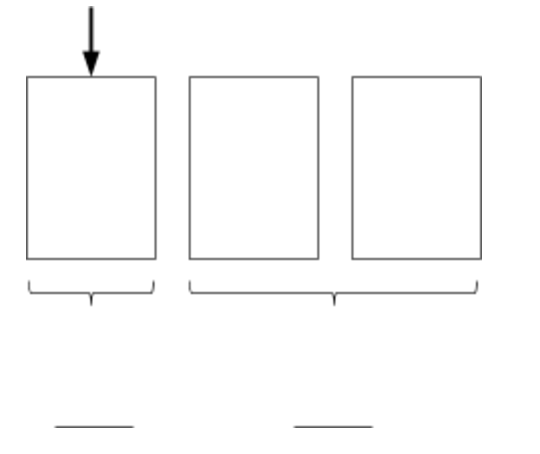
\includegraphics[width=8cm, height=6cm]{intro_doors_1.jpg}
\end{center}
\begin{solution}
\begin{center}
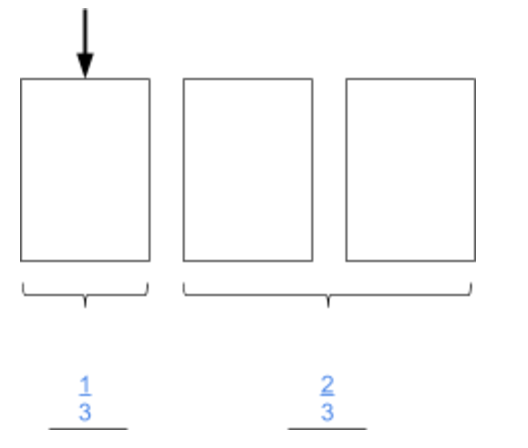
\includegraphics[width=5cm, height=5.5cm]{intro_doors_1_sol.jpg}
\end{center}
 \end{solution}
 
After the host opens a door with a goat, what are the probabilities of 
the car being behind each door?
\begin{center}
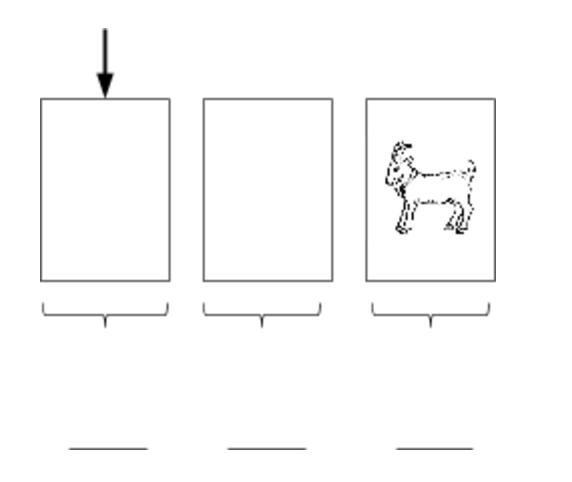
\includegraphics[width=8cm, height=5.5cm]{intro_doors_2.jpg}
\end{center}
\begin{solution}
\begin{center}
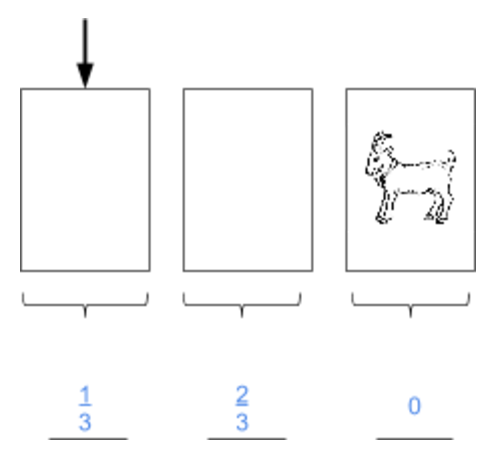
\includegraphics[width=5cm, height=4cm]{intro_doors_2_sol.jpg}
\end{center}
 \end{solution}
 
 These probabilities might initially seem counterintuitive, but can be explained through an important probability theorem, Bayes' rule, which says that:
 \[ \P[A|B] = \frac{\P[B|A]P[A]}{\P[B]} \]
 We can apply this rule to the Monty Hall problem, as shown in the figure below. We assume that the contestant has chosen Door A. \newline
 \begin{figure}[!ht]
\caption{From ucanalytics.com}
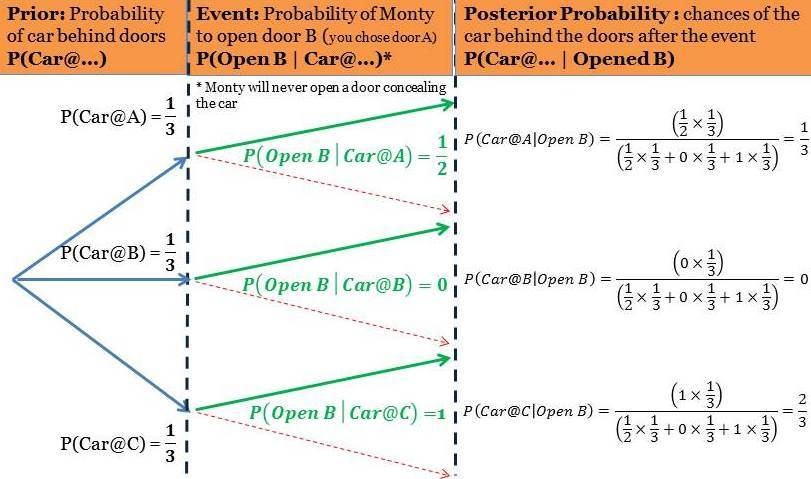
\includegraphics[width=17cm, height=10cm]{BayesRuleMontyHall.jpg}
\end{figure}
\newline 
Beyond Monty Hall, Bayes' rule can be applied to a wide variety of problems, as will be shown in the next section on conditional probability. 
